\begin{solution}
$f(x)=x+1$
\begin{itemize}
\item Pente :	 
\item Ordonnée à l’origine :	$x=0\Rightarrow f(x)=1$ 
\item Zéro de fonction :	$f(x)=0\Rightarrow x=-1$
\item Signe et variation :	
$$\begin{array}{l|l|l|l|l|l}
x    & -\infty &   & -1 &   & +\infty \\
\hline
f(x) & -       & - & 0  & + & +   \\
 & -\infty & \nearrow & \nearrow & \nearrow & +\infty \\   
\end{array}$$
\item Graphique
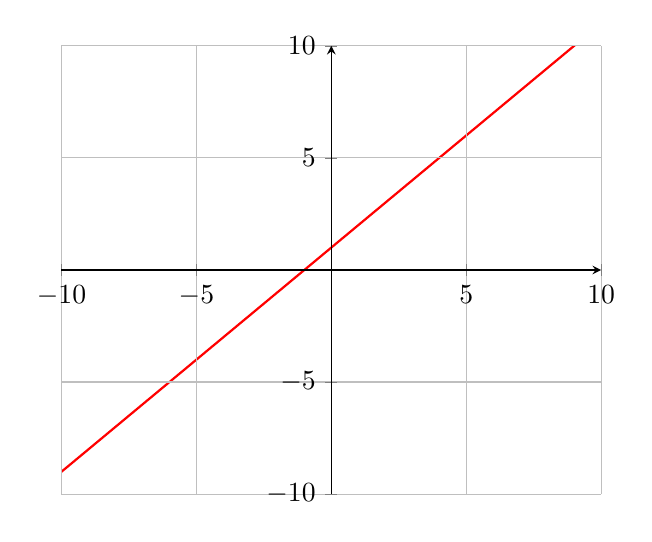
\begin{tikzpicture}
\begin{axis}[
	grid= major,
    xmin=-10, xmax=10,
    ymin=-10, ymax=10,
    axis lines=center,
    axis on top=true,
    domain=-10:10,
    ]

    \addplot [mark=none,draw=red, thick] {x+1};
\end{axis}
\end{tikzpicture}
\end{itemize}
\end{solution}

\begin{solution}
$f(x)=x-3$
\begin{itemize}
\item Pente :	$a=1$
\item Ordonnée à l’origine :	$x=0\Rightarrow f(x)=-3$
\item Zéro de fonction :	$f(x)=0\Rightarrow x=3$
\item Signe :	
$$\begin{array}{l|l|l|l|l|l}
x    & -\infty &   & 3 &   & +\infty \\
\hline
f(x) & -       & - & 0  & + & +      \\
& -\infty & \nearrow & \nearrow & \nearrow & +\infty \\   
\end{array}$$
\item Graphique
\begin{tikzpicture}
\begin{axis}[
    xmin=-10, xmax=10,
    ymin=-10, ymax=10,
    axis lines=center,
    axis on top=true,
    domain=-10:10,
    ]

    \addplot [mark=none,draw=red, thick] {x-3};
\end{axis}
\end{tikzpicture}
\end{itemize}
\end{solution}

\begin{solution}
$f(x)=2x-3$
\begin{itemize}
\item Pente :	$a=2$
\item Ordonnée à l’origine :	$x=0\Rightarrow f(x)=-3$
\item Zéro de fonction :	$f(x)=0\Rightarrow x=\frac{3}{2}$
\item Signe :	
$$\begin{array}{l|l|l|l|l|l}
x    & -\infty &   & \frac{3}{2} &   & +\infty \\
\hline
f(x) & -       & - & 0  & + & +      
\end{array}$$
\item Graphique
\begin{tikzpicture}
\begin{axis}[
    xmin=-10, xmax=10,
    ymin=-10, ymax=10,
    axis lines=center,
    axis on top=true,
    domain=-10:10,
    ]

    \addplot [mark=none,draw=red, thick] {2*x-3};
\end{axis}
\end{tikzpicture}
\end{itemize}
\end{solution}

\begin{solution}
$f(x)=2x+5$
\begin{itemize}
\item Pente :	$a=2$
\item Ordonnée à l’origine :	$x=0\Rightarrow f(x)=5$
\item Zéro de fonction :	$f(x)=0\Rightarrow x=-\frac{5}{2}$
\item Signe :	
$$\begin{array}{l|l|l|l|l|l}
x    & -\infty &   & -\frac{5}{2} &   & +\infty \\
\hline
f(x) & -       & - & 0  & + & +   \\
 & -\infty & \nearrow & \nearrow & \nearrow & +\infty \\   
\end{array}$$
\item Graphique
\begin{tikzpicture}
\begin{axis}[
    xmin=-10, xmax=10,
    ymin=-10, ymax=10,
    axis lines=center,
    axis on top=true,
    domain=-10:10,
    ]

    \addplot [mark=none,draw=red, thick] {2*x+5};
\end{axis}
\end{tikzpicture}
\end{itemize}
\end{solution}

\begin{solution}
$f(x)=\frac{x}{2}+1$
\begin{itemize}
\item Pente :	$a=\frac{1}{2}$
\item Ordonnée à l’origine :	$x=0\Rightarrow f(x)=1$
\item Zéro de fonction :	$f(x)=0\Rightarrow x=-2$
\item Signe :	
$$\begin{array}{l|l|l|l|l|l}
x    & -\infty &   & -2 &   & +\infty \\
\hline
f(x) & -       & - & 0  & + & +   \\
 & -\infty & \nearrow & \nearrow & \nearrow & +\infty \\   
\end{array}$$
\item Graphique
\begin{tikzpicture}
\begin{axis}[
    xmin=-10, xmax=10,
    ymin=-10, ymax=10,
    axis lines=center,
    axis on top=true,
    domain=-10:10,
    ]

    \addplot [mark=none,draw=red, thick] {x/2+1};
\end{axis}
\end{tikzpicture}
\end{itemize}
\end{solution}

\begin{solution}
$f(x)=-x+1$
\begin{itemize}
\item Pente :	$a=-1$
\item Ordonnée à l’origine :	$x=0\Rightarrow f(x)=1$
\item Zéro de fonction :	$f(x)=0\Rightarrow x=1$
\item Signe :
$$\begin{array}{l|l|l|l|l|l}
x    & -\infty &   & 1 &   & +\infty \\
\hline
f(x) & +       & + & 0  & - & -   \\
 & +\infty & \searrow & \searrow & \searrow & -\infty \\   
\end{array}$$
\item Graphique
\begin{tikzpicture}
\begin{axis}[
    xmin=-10, xmax=10,
    ymin=-10, ymax=10,
    axis lines=center,
    axis on top=true,
    domain=-10:10,
    ]

    \addplot [mark=none,draw=red, thick] {-x+1};
\end{axis}
\end{tikzpicture}
\end{itemize}
\end{solution}

\begin{solution}
$f(x)=-x-3$
\begin{itemize}
\item Pente :	$a=-1$
\item Ordonnée à l’origine :	$x=0\Rightarrow f(x)=-3$
\item Zéro de fonction :	$f(x)=0\Rightarrow x=-3$
\item Signe :	
$$\begin{array}{l|l|l|l|l|l}
x    & -\infty &   & -3 &   & +\infty \\
\hline
f(x) & +       & + & 0  & - & -   \\
 & +\infty & \searrow & \searrow & \searrow & -\infty \\   
\end{array}$$
\item Graphique
\begin{tikzpicture}
\begin{axis}[
    xmin=-10, xmax=10,
    ymin=-10, ymax=10,
    axis lines=center,
    axis on top=true,
    domain=-10:10,
    ]

    \addplot [mark=none,draw=red, thick] {-x-3};
\end{axis}
\end{tikzpicture}
\end{itemize}
\end{solution}

\begin{solution}
$f(x)=-2x-3$
\begin{itemize}
\item Pente :	$a=-2$
\item Ordonnée à l’origine :	$x=0\Rightarrow f(x)=-3$
\item Zéro de fonction :	$f(x)=0\Rightarrow x=-\frac{3}{2}$
\item Signe :	
$$\begin{array}{l|l|l|l|l|l}
x    & -\infty &   & -\frac{3}{2} &   & +\infty \\
\hline
f(x) & +       & + & 0  & - & -   \\
 & +\infty & \searrow & \searrow & \searrow & -\infty \\   
\end{array}$$
\item Graphique
\begin{tikzpicture}
\begin{axis}[
    xmin=-10, xmax=10,
    ymin=-10, ymax=10,
    axis lines=center,
    axis on top=true,
    domain=-10:10,
    ]

    \addplot [mark=none,draw=red, thick] {-2*x-3};
\end{axis}
\end{tikzpicture}
\end{itemize}
\end{solution}

\begin{solution}
$f(x)=5x+8$
\begin{itemize}
\item Pente :	$a=5$
\item Ordonnée à l’origine :	$x=0\Rightarrow f(x)=8$ 
\item Zéro de fonction :	$f(x)=0\Rightarrow x=-\frac{8}{5}$
\item Signe :
$$\begin{array}{l|l|l|l|l|l}
x    & -\infty &   & -\frac{8}{5} &   & +\infty \\
\hline
f(x) & -       & - & 0  & + & +   \\
 & -\infty & \nearrow & \nearrow & \nearrow & +\infty \\   
\end{array}$$
\item Graphique
\begin{tikzpicture}
\begin{axis}[
    xmin=-10, xmax=10,
    ymin=-10, ymax=10,
    axis lines=center,
    axis on top=true,
    domain=-10:10,
    ]

    \addplot [mark=none,draw=red, thick] {5*x+8};
\end{axis}
\end{tikzpicture}
\end{itemize}
\end{solution}

\begin{solution}
$f(x)=\frac{2x}{5}-3$
\begin{itemize}
\item Pente :	$a=\frac{2}{5}$
\item Ordonnée à l’origine :	$x=0\Rightarrow f(x)=-3$ 
\item Zéro de fonction :	$f(x)=0\Rightarrow x=\frac{15}{2}$
\item Signe :
$$\begin{array}{l|l|l|l|l|l}
x    & -\infty &   & -\frac{15}{2} &   & +\infty \\
\hline
f(x) & -       & - & 0  & + & +   \\
 & -\infty & \nearrow & \nearrow & \nearrow & +\infty \\   
\end{array}$$
\item Graphique
\begin{tikzpicture}
\begin{axis}[
    xmin=-10, xmax=10,
    ymin=-10, ymax=10,
    axis lines=center,
    axis on top=true,
    domain=-10:10,
    ]

    \addplot [mark=none,draw=red, thick] {2*x/5-3};
\end{axis}
\end{tikzpicture}
\end{itemize}
\end{solution}

\begin{solution}
$f(x)=5x-5$
\begin{itemize}
\item Pente :	$a=5$
\item Ordonnée à l’origine :	$x=0\Rightarrow f(x)=-5$ 
\item Zéro de fonction :	$f(x)=0\Rightarrow x=1$
\item Signe :
$$\begin{array}{l|l|l|l|l|l}
x    & -\infty &   & 1 &   & +\infty \\
\hline
f(x) & -       & - & 0  & + & +   \\
 & -\infty & \nearrow & \nearrow & \nearrow & +\infty \\   
\end{array}$$
\item Graphique
\begin{tikzpicture}
\begin{axis}[
    xmin=-10, xmax=10,
    ymin=-10, ymax=10,
    axis lines=center,
    axis on top=true,
    domain=-10:10,
    ]

    \addplot [mark=none,draw=red, thick] {5*x-5};
\end{axis}
\end{tikzpicture}
\end{itemize}
\end{solution}

\begin{solution}
$f(x)=-10x+3$
\begin{itemize}
\item Pente :	$a=-10$
\item Ordonnée à l’origine :	$x=0\Rightarrow f(x)=3$
\item Zéro de fonction :	$f(x)=0\Rightarrow x=\frac{3}{10}$
\item Signe :	
$$\begin{array}{l|l|l|l|l|l}
x    & -\infty &   & \frac{3}{10} &   & +\infty \\
\hline
f(x) & +       & + & 0  & - & -   \\
 & +\infty & \searrow & \searrow & \searrow & -\infty \\   
\end{array}$$
\item Graphique
\begin{tikzpicture}
\begin{axis}[
    xmin=-10, xmax=10,
    ymin=-10, ymax=10,
    axis lines=center,
    axis on top=true,
    domain=-10:10,
    ]

    \addplot [mark=none,draw=red, thick] {-10*x+3};
\end{axis}
\end{tikzpicture}
\end{itemize}
\end{solution}

\begin{solution}
$f(x)=-3x+7$
\begin{itemize}
\item Pente :	$a=-3$
\item Ordonnée à l’origine :	$x=0\Rightarrow f(x)=7$
\item Zéro de fonction :	$f(x)=0\Rightarrow x=\frac{7}{3}$
\item Signe :
$$\begin{array}{l|l|l|l|l|l}
x    & -\infty &   & \frac{7}{3} &   & +\infty \\
\hline
f(x) & +       & + & 0  & - & -   \\
 & +\infty & \searrow & \searrow & \searrow & -\infty \\   
\end{array}$$
\item Graphique
\begin{tikzpicture}
\begin{axis}[
    xmin=-10, xmax=10,
    ymin=-10, ymax=10,
    axis lines=center,
    axis on top=true,
    domain=-10:10,
    ]

    \addplot [mark=none,draw=red, thick] {-3*x+7};
\end{axis}
\end{tikzpicture}
\end{itemize}
\end{solution}

\begin{solution}
$f(x)=\frac{3}{8}x-2$
\begin{itemize}
\item Pente :	$a=\frac{3}{8}$
\item Ordonnée à l’origine :	$x=0\Rightarrow f(x)=-2$ 
\item Zéro de fonction :	$f(x)=0\Rightarrow x=\frac{16}{3}$
\item Signe :	
$$\begin{array}{l|l|l|l|l|l}
x    & -\infty &   & \frac{16}{3} &   & +\infty \\
\hline
f(x) & -       & - & 0  & + & +   \\
 & -\infty & \nearrow & \nearrow & \nearrow & +\infty \\   
\end{array}$$
\item Graphique
\begin{tikzpicture}
\begin{axis}[
    xmin=-10, xmax=10,
    ymin=-10, ymax=10,
    axis lines=center,
    axis on top=true,
    domain=-10:10,
    ]

    \addplot [mark=none,draw=red, thick] {3*x/8-2};
\end{axis}
\end{tikzpicture}
\end{itemize}
\end{solution}

\begin{solution}
$f(x)=-\frac{x}{8}-1$
\begin{itemize}
\item Pente :	$a=-\frac{1}{8}$
\item Ordonnée à l’origine :	$x=0\Rightarrow f(x)=-1$
\item Zéro de fonction :	$f(x)=0\Rightarrow x=-8$
\item Signe :	
$$\begin{array}{l|l|l|l|l|l}
x    & -\infty &   & -8 &   & +\infty \\
\hline
f(x) & +       & + & 0  & - & -   \\
 & +\infty & \searrow & \searrow & \searrow & -\infty \\   
\end{array}$$
\item Graphique
\begin{tikzpicture}
\begin{axis}[
    xmin=-10, xmax=10,
    ymin=-10, ymax=10,
    axis lines=center,
    axis on top=true,
    domain=-10:10,
    ]

    \addplot [mark=none,draw=red, thick] {-x/8-1};
\end{axis}
\end{tikzpicture}
\end{itemize}
\end{solution}

\begin{solution}
$f(x)=5$
\begin{itemize}
\item Pente :	$a=0$
\item Ordonnée à l’origine :	$x=0\Rightarrow f(x)=5$
\item Zéro de fonction :	$f(x)=0\Rightarrow x=\pm \infty $
\item Signe :	$$\begin{array}{l|l|l|l|l|l}
x    & -\infty &   & &   & +\infty \\
\hline
f(x) & +       & + & +  & + & +   \\
 & 5 & \rightarrow & \rightarrow & \rightarrow & 5 \\   
\end{array}$$
\item Graphique
\begin{tikzpicture}
\begin{axis}[
    xmin=-10, xmax=10,
    ymin=-10, ymax=10,
    axis lines=center,
    axis on top=true,
    domain=-10:10,
    ]

    \addplot [mark=none,draw=red, thick] {5};
\end{axis}
\end{tikzpicture}
\end{itemize}
\end{solution}

\begin{solution}
$f(x)=-4$
\begin{itemize}
\item Pente :	$a=0$
\item Ordonnée à l’origine :	$x=0\Rightarrow f(x)=-4$
\item Zéro de fonction :	$f(x)=0\Rightarrow x=\pm \infty $
\item Signe :	$$\begin{array}{l|l|l|l|l|l}
x    & -\infty &   & &   & +\infty \\
\hline
f(x) & -       & - & -  & - & -   \\
 & -4 & \rightarrow & \rightarrow & \rightarrow & -4 \\   
\end{array}$$
\item Graphique
\begin{tikzpicture}
\begin{axis}[
    xmin=-10, xmax=10,
    ymin=-10, ymax=10,
    axis lines=center,
    axis on top=true,
    domain=-10:10,
    ]

    \addplot [mark=none,draw=red, thick] {-4};
\end{axis}
\end{tikzpicture}
\end{itemize}
\end{solution}

\begin{solution}
$f(x)=3x$
\begin{itemize}
\item Pente :	$a=3$
\item Ordonnée à l’origine :	$x=0\Rightarrow f(x)=0$ 
\item Zéro de fonction :	$f(x)=0\Rightarrow x=0$
\item Signe :	$$\begin{array}{l|l|l|l|l|l}
x    & -\infty &   & 0 &   & +\infty \\
\hline
f(x) & -       & - & 0  & + & +   \\
 & -\infty & \nearrow & \nearrow & \nearrow & +\infty \\   
\end{array}$$
\item Graphique
\begin{tikzpicture}
\begin{axis}[
    xmin=-10, xmax=10,
    ymin=-10, ymax=10,
    axis lines=center,
    axis on top=true,
    domain=-10:10,
    ]

    \addplot [mark=none,draw=red, thick] {3*x};
\end{axis}
\end{tikzpicture}
\end{itemize}
\end{solution}

\begin{solution}
$f(x)=-6x$
\begin{itemize}
\item Pente :	$a=-6$
\item Ordonnée à l’origine :	$x=0\Rightarrow f(x)=0$
\item Zéro de fonction :	$f(x)=0\Rightarrow x=0$
\item Signe :	$$\begin{array}{l|l|l|l|l|l}
x    & -\infty &   & 0 &   & +\infty \\
\hline
f(x) & +       & + & 0  & - & -   \\
 & +\infty & \searrow & \searrow & \searrow & -\infty \\   
\end{array}$$
\item Graphique
\begin{tikzpicture}
\begin{axis}[
    xmin=-10, xmax=10,
    ymin=-10, ymax=10,
    axis lines=center,
    axis on top=true,
    domain=-10:10,
    ]

    \addplot [mark=none,draw=red, thick] {-6*x};
\end{axis}
\end{tikzpicture}
\end{itemize}
\end{solution}

\begin{solution}
$f(x)=\frac{5}{7}x$
\begin{itemize}
\item Pente :	$a=\frac{5}{7}$
\item Ordonnée à l’origine :	$x=0\Rightarrow f(x)=0$ 
\item Zéro de fonction :	$f(x)=0\Rightarrow x=0$
\item Signe :	$$\begin{array}{l|l|l|l|l|l}
x    & -\infty &   & 0 &   & +\infty \\
\hline
f(x) & -       & - & 0  & + & +   \\
 & -\infty & \nearrow & \nearrow & \nearrow & +\infty \\   
\end{array}$$
\item Graphique
\begin{tikzpicture}
\begin{axis}[
    xmin=-10, xmax=10,
    ymin=-10, ymax=10,
    axis lines=center,
    axis on top=true,
    domain=-10:10,
    ]

    \addplot [mark=none,draw=red, thick] {5*x/7};
\end{axis}
\end{tikzpicture}
\end{itemize}
\end{solution}

